\documentclass[12pt]{article}
\usepackage[letterpaper, margin=1in]{geometry}
\usepackage{graphicx}
\usepackage{subcaption}
\graphicspath{{./Figures/}}
\usepackage{hyperref}
\usepackage{parskip}

\title{ELECENG 3CL4 Lab 1}
\author{
    Aaron Pinto \\
    pintoa9 \\
    L02
    \and
    Raeed Hassan \\
    hassam41 \\
    L02
}

\begin{document}

\maketitle
\clearpage

\section*{Member Contributions}
Both group members contributed an even amount to both the exercises and the report. Both members went through the exercises together and contributed to all sections of the report.

\section*{Simulation Environment}
The software used for our simulation environment consisted of Microsoft Windows 10 Education (Version 20H2, OS Build 19042.746), MATLAB R2020b Update 3, and Quanser Interactive Labs Version 2.9. This software was run on a Dell laptop with an Intel Core i7-8550U processor, 8GB of DDR4-2400MHz RAM, Intel UHD Graphics 620 (integrated), and a 256GB SSD.

\section*{Familiarization Exercises} % might change subsection tiles, just leave it like this for now
% name them subsection_voltage and subsection_angle (eg vii_voltage/vii_angle)
% don't worry about the figure placement, it'll probably fix itself once you add more text or i'll fix it later

\subsection*{Initial setup} % base settings, vii/viii
The initial exercise had the proportional gain set to 1 and the derivative gain set to 0. The motor voltage quickly increased to just under 2 V and quickly shot back down, but required some time to settle back to 0 V. Figure~\ref{fig:vii_volt} shows a plot of the motor voltage. The servo angle shoots past the 45 degrees to almost 80 degrees, before beginning to settle towards 45 degrees. The servo angle settles a bit under the targeted 45 degrees. Figure~\ref{fig:vii_angle} shows a plot of the servo angle.
\begin{figure}[h!]
    \centering
    \begin{subfigure}[b]{0.46\textwidth}
        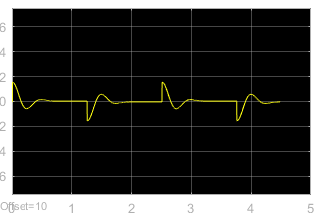
\includegraphics[width=\textwidth]{vii_voltage}    
        \caption{\label{fig:vii_volt}Motor Voltage}    
    \end{subfigure}
    \begin{subfigure}[b]{0.46\textwidth}
        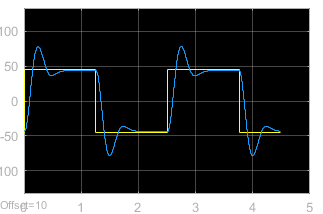
\includegraphics[width=\textwidth]{vii_angle}
        \caption{\label{fig:vii_angle}Servo Angle}
    \end{subfigure}
    \caption{\label{fig:vii}Proportional gain: 1, Derivative gain = 0}
\end{figure}

\subsection*{Investigating the Effects of Increasing Proportional Gain} % increase proportional gain 1 -> 2, ix
In the following familiarization exercise, the proportional gain is set to 2. We observe even greater overshoot, with more oscillations before the motor voltage and servo angle settle. The motor voltage spikes to approximately 3 V now, as a result of it being driven harder by the bigger proportional gain, but requires longer to settle down to 0 V. Figure~\ref{fig:ix_volt} shows a plot of the motor voltage. Similarly, the servo angle jumps to almost 100 degrees this time, before requiring a longer amount of time to settle to 45 degrees. However, the servo angle does eventually settle down to 45 degrees. Figure~\ref{fig:ix_angle} shows a plot of the servo angle.
\begin{figure}[h!]
    \centering
    \begin{subfigure}[b]{0.46\textwidth}
        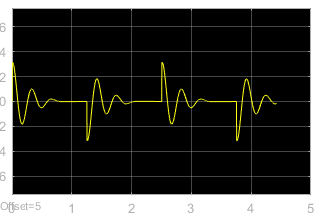
\includegraphics[width=\textwidth]{ix_voltage}
        \caption{\label{fig:ix_volt}Motor Voltage}
    \end{subfigure}
    \begin{subfigure}[b]{0.46\textwidth}
        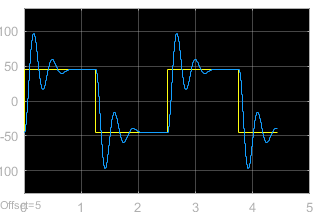
\includegraphics[width=\textwidth]{ix_angle}
        \caption{\label{fig:ix_angle}Servo Angle}
    \end{subfigure}
    \caption{\label{fig:ix} Proportional gain: 2, Derivative gain = 0}
\end{figure}

% \subsection*{x} % increase proportional gain 2 -> 4, x
Increasing the proportional gain further to 4 causes even greater overshoot, and even more oscillations as the settling time increases significantly. The motor voltage spikes all the way up to 6 V and oscillates for the entire period. The motor is driven in the other direction before it even has a chance to settle. Figure~\ref{fig:x_volt} shows a plot of the motor voltage. Similarly, the servo angle overshoots the targeted angle even farther, and does not even have enough time to settle at 45 degrees before it is driven the other way. Figure~\ref{fig:x_angle} shows a plot of the servo angle.
\begin{figure}[h!]
    \centering
    \begin{subfigure}[b]{0.46\textwidth}
        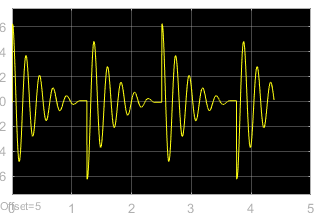
\includegraphics[width=\textwidth]{x_voltage}
        \caption{\label{fig:x_volt}Motor Voltage}
    \end{subfigure}
    \begin{subfigure}[b]{0.46\textwidth}
        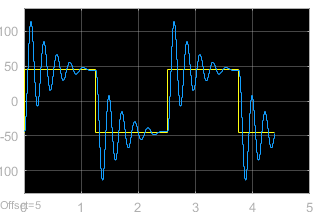
\includegraphics[width=\textwidth]{x_angle}
        \caption{\label{fig:x_angle}Servo Angle}
    \end{subfigure}
    \caption{\label{fig:x} Proportional gain: 4, Derivative gain = 0}
\end{figure}

\subsection*{Introducing Derivative Gain} % increase derivative gain 0 -> 0.1, xi
In the next familiarization exercise, we add a derivative gain by increasing it from 0 to 0.15 while keeping the proportional gain at 4. The motion of the disk is much smoother with little overshoot and a very short period of oscillations. The motor voltage still peaks at around 6 V but the subsequent peak was much smaller at 2 V, with oscillations stopping very quickly and the motor remaining settled for the majority of the period. Figure~\ref{fig:xi_volt} shows a plot of the motor voltage. The servo angle only shoots a bit over the desired angle, but settles down near the desired angle very quickly. The angle remains slightly under 45 degrees for most of the period. Figure~\ref{fig:xi_angle} shows a plot of the servo angle.
\begin{figure}[h!]
    \centering
    \begin{subfigure}[b]{0.46\textwidth}
        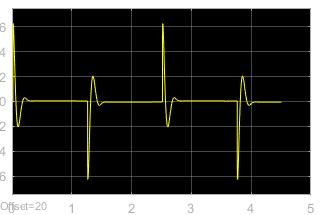
\includegraphics[width=\textwidth]{xi_voltage}
        \caption{\label{fig:xi_volt}Motor Voltage}
    \end{subfigure}
    \begin{subfigure}[b]{0.46\textwidth}
        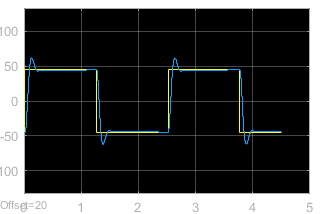
\includegraphics[width=\textwidth]{xi_angle}
        \caption{\label{fig:xi_angle}Servo Angle}    
    \end{subfigure}
    \caption{\label{fig:xi} Proportional gain: 4, Derivative gain = 0.1}
\end{figure}

\subsection*{Investigating the Effects of Increasing Derivative Gain} % increase derivative gain 0.1 -> 0.15, xii
Increasing the derivative gain further to 0.15 causes the motion to be even smoother. The durations of the peaks in the motor voltage are even tighter than before. Figure~\ref{fig:xii_volt} shows a plot of the motor voltage. The servo angle arrives at 45 degrees much quicker than previously. Figure~\ref{fig:xii_angle} shows a plot of the servo angle. We can observe that increasing the derivative gain decreases the overshoot and requires less correction.
\begin{figure}[h!]
    \centering
    \begin{subfigure}[b]{0.46\textwidth}
        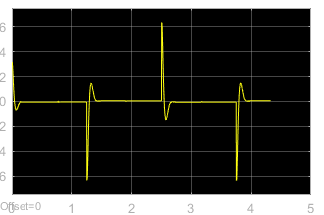
\includegraphics[width=\textwidth]{xii_voltage}
        \caption{\label{fig:xii_volt}Motor Voltage}     
    \end{subfigure}
    \begin{subfigure}[b]{0.46\textwidth}
        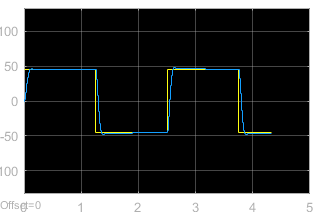
\includegraphics[width=\textwidth]{xii_angle}
        \caption{\label{fig:xii_angle}Servo Angle} 
    \end{subfigure}
    \caption{\label{fig:xii} Proportional gain: 4, Derivative gain = 0.15}
    %\vspace{128in} % added to push figure to top of page
\end{figure}
\end{document}
